\documentclass[a4paper, 10pt]{article}
\usepackage{INTERSPEECH2021}

\usepackage{amsmath,amssymb,amsfonts}
\usepackage[hidelinks]{hyperref}
\usepackage{cleveref}
\usepackage{graphicx, floatrow}
\usepackage{enumitem}

\DeclareFloatSeparators{Qquad}{\hskip2em}

% args: big, bigg, Big, Bigg
\newcommand{\parenth}[2][]{#1(#2#1)}
\renewcommand{\bold}[1]{\textbf{\structure{#1}}}

\title{Adopting and improving LSTMs as Language models}
\name{Filippo Daniotti (232087)}

\address{
  University of Trento}
\email{filippo.daniotti@studenti.unitn.it}

\begin{document}

\maketitle

% Dear students, \\
% here you can find a complete description of the sections that are mandatory for your project and you need to address them during the development, as well as your 4-page (+1 for References) project report.


\section{Introduction}
% approx. 100 words
This document is the final report for the course \emph{Natural Language Understanding} of the Master's Degree in Artificial Intelligence Systems at the University of Trento in the A.Y.2021/2022. The goal of the project is to implement a language model based on LSTMs\cite{hochreiter1997lstm} and to evaluate its performances on the word-level Penn Treebank\cite{marcus1993building} dataset and achieve a perplecity score $\le 90.7$. In this work:
\begin{itemize}
    \item we analyzed the dataset;
    \item we implemented and trained a baseline LSTM model and a refined regularized LSTM model;
    \item we fine-tuned the refined model and improved it with additional regularization techniques from the literature;
    \item we evaluated the models and performed an in-depth analysis of the best performing model behaviour;
    \item we created a TUI application to easily interact with the model and use it to generate sentences.
\end{itemize}
The final model achieved a perplexity score of $79.86$ on the test set. The code for this project is available at \url{https://github.com/filippodaniotti/NLU-UniTN-2022}
\section{Task Formalisation}
% approx. 200 words
Language modelling is the task of developing a model which is able to predict which word comes next in a sequence. 

A \emph{language model} is a probablity distribution over sequences of words. Suppose we have a sequence of \(n\) words modeled as a joint probability: \(P(w^{(n)}) = P(w_1, \ldots, w_n)\); we can compute this probablity using the \emph{chain rule}, which comes from the Bayes rule: \(P(A, B) = P(A|B)P(B)\). Ultimately, a language model computes the probability of a sequence as follows:

\begin{equation}
    P(w_1, \ldots, w_n)  = \prod_{k=1}^{n}P \parenth[\bigg]{w_k|w_1^{(k-1)}}
\end{equation}

The underlying assumption is that sentences in natural languages have \emph{structure}, hence we can compute the joint distribution from data, i.e. \emph{corpora}. However, this setting is challenged by several properties of natural languages. Although we can trace some general schemes for structure - e.g. word orders like VSO, SVO, \emph{et cetera} - natural languages allow non-standard phrasing; moreover, they allow sentences to grow up to arbitrary lengths. More generally, we will never be able to compute statistics for the sentences space, which is unbounded for what concerns our task.

To cope with this problem, we can compute statistics for a word considering a small window of preceeding words. Formally, motivated by the Markov Assumption, we think of this process as mapping the original space into a smaller one, for which we can easily compute statistics: these language models are called \emph{n}-gram language models, and they usually consider bigram probabilities - \(P \parenth[\big]{w_i | w_1^{(i-1)}} \approx P \parenth[\big]{w_i | w_{i-1}}\) - or trigram probabilities - \(P\parenth[\big]{w_i | w_1^{(i-1)}} \approx P \parenth[\big]{w_i | w_{i-2}^{(i-1)}}\).

Currently, state-of-the-art language models are \emph{Neural language models}, i.e. language models that use neural network models to perform embeddings and approximate the distribution. In particular, the first effective models to be employed where Recurrent Neural Networks, such as LSTMs and GRUs; last developments revolve around attention-based models, and specifically Transformers. 

\section{Data Description \& Analysis}
\label{sec:3_data}
% approx. 200-500 words
\paragraph*{Description}
The dataset used to train and evaluate the model is word-level Penn Treebank\cite{marcus1993building}, which is a variation of the original Penn Treebank dataset built to be best suited to language modelling settings. 

Specifically, the original Penn Treebank has undergone a pre-processing pipeline so that it features:

\begin{itemize}
    \item consistent lowercase;
    \item tokenization;
    \item no punctuation;
    \item proper nouns and other rare words have been encompassed by a \texttt{<unk>} token;
    \item digits have been replaced with a \texttt{N} token;
    \item no OOV words in \emph{validation} and \emph{test} sets with respect to the \emph{training} set.
\end{itemize}

\begin{table}
    \begin{tabular}{lccc}
    \toprule
    & \textbf{Train} & \textbf{Validation} & \textbf{Test} \\
    \midrule
    Sents split percentage & 
    \(85.51\)\% & \(6.85\)\% & \(7.64\)\%  \\
    Words split percentage & 
    \(85.62\)\% & \(6.79\)\% & \(7.59\)\%  \\
    \# Sentences & 
    \(42,068\) & \(3,370\) & \(3,761\) \\
    \# Words & 
    \(887,521\) & \(70,390\) & \(78,669\) \\ 
    \# Vocabulary & 
    \(9,999\) & \(6,021\) & \(6,048\) \\
    \# OOV words & 
    - & \(0\) & \(0\) \\
    \midrule
    Sentence lengths mean & 
    \(20.09\) & \(20.88\) & \(20.91\) \\
    Sentence lengths median & 
    \(20.0\) & \(20.0\) & \(20.0\) \\
    Sentence lengths \(\sigma\) &
    \(10.14\) & \(9.98\) & \(10.18\) \\
    Sentence max length & 
    \(82\) & \(74\) & \(77\) \\
    Sentence min length & 
    \(1\) & \(1\) & \(1\) \\

    \bottomrule
\end{tabular}
    \caption{Statistics of word-level Penn Treebank}
    \label{tab:statistics}
\end{table}

\paragraph*{Statistics analysis}
In Tab.\ref{tab:statistics} we are presenting a summary of the relevant statistics of the dataset.

The PTB dataset appears to be balanced enough, as sents and words are evenly splitted and the mean and standard deviance \(\sigma\) of the words-per-sentence distribution are very similar, being around \(20\) and \(10\).

Moreover, since there are no OOV words, we can rely on the train split to construct the vocabulary. Its length is given by the \(9999\) words, to which we added two additional tokens:
\begin{itemize}
    \item \texttt{<pad>} is a pad token to pad shorter sequences to the length of the longest sequence in a given batch;
    \item \texttt{<eos>} is a sentence terminator token.
\end{itemize}

The analysis of the most frequent words in the train split reveals that the most frequent words are extremely common function words, like articles (\textit{the}, \(5.7\)\%), or prepositions (\textit{of}, \(2.7\)\%), which is unsurprising. We are not surprised to observe that the two wrappers \texttt{<unk>} and \texttt{N} show high counts, being \(5.1\)\% and \(3.7\)\% respectively, ranking second and third most frequent words. Ultimately, the first 10 most frequent words make up almost 30\% of the total word count.

\begin{figure}[!t]
    \centering
    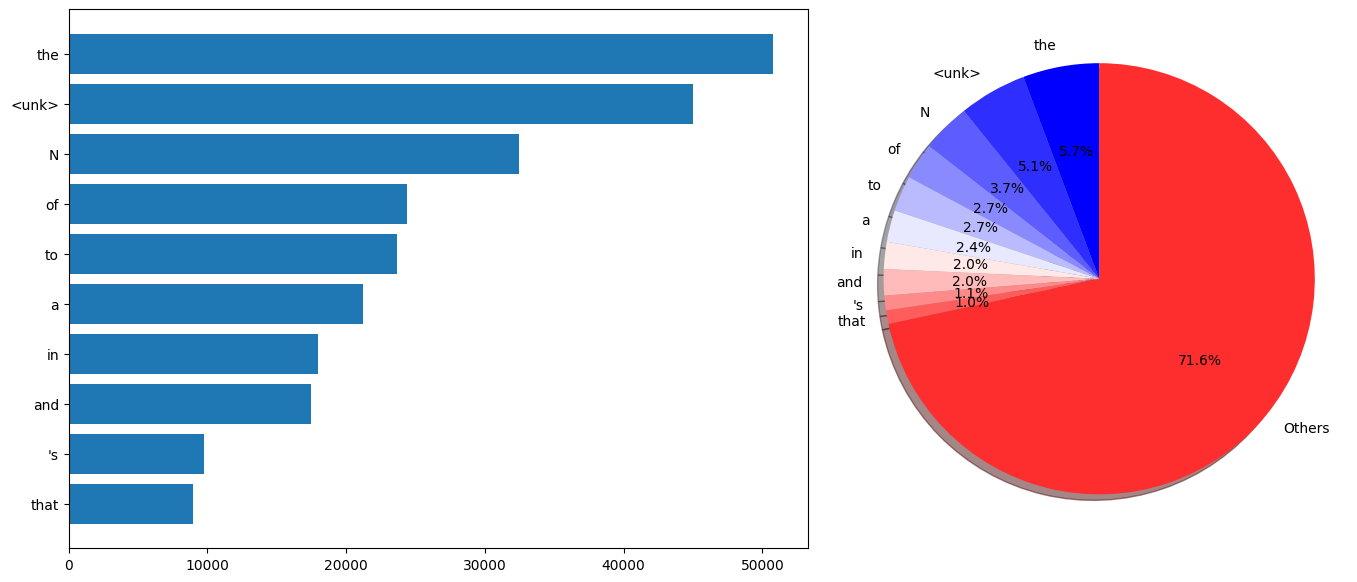
\includegraphics[keepaspectratio,width=\textwidth]{assets/images/train_freq.png}
    \caption{Frequency distribution of the 10 most frequent words (Train)} 
    \label{fig:train_freq}
\end{figure}

\section{Model}
\label{sec:4_model}
% approx. 200-500 words
% \begin{itemize}
%     \item \textit{your network/ algorithm (do not spend too much text in explaining already existing models, focus on your solution),}
%     \item \textit{the pipeline if used any, including  tokenizer, featurizer, extractor, etc.}
%     \item \textit{Your baseline and the experiments you have tried}
% \end{itemize}
 
\subsection{Architecture}
\label{sec:4_arch}
We employed LSTMs\cite{hochreiter1997lstm} as backbone architecture, as they outperform Vanilla RNNs and GRUs in caputirng long-term dependencies, which is a key feature for language modelling. The model features the following components:
\begin{itemize}
    \item a \emph{word embedding} layer, which maps the input words to a sparse vector representation;
    \item a \emph{recurrent LSTM} layer, which processes the sequence of embeddings and outputs a sequence of hidden states;
    \item a \emph{fully-connected} layer, which maps the hidden states to a sequence of logits.
\end{itemize}
We have implemented two different architectures:
\begin{itemize}
    \item \emph{Baseline LSTM}: baseline model with a single-layer LSTM with \(300\) hidden units;
    \item \emph{Merity LSTM}: refined architecture featuring a set of regularization technique, which will be discussed later.
\end{itemize}

\subsection{Pipeline}
The complete experiment pipeline is structured as follows.
\begin{enumerate}
    \item \emph{Data loading}: the dataset is downloaded, extracted and loaded into memory.
    \item \emph{Data pre-processing}: in order to be ready to be fed to the model, the following operations are performed:
    \begin{itemize} 
        \item each sentence is tokenized by splitting on whitespaces;
        \item a \texttt{<eos>} token is appended to each sentence;
        \item the vocabulary mappings are created.
    \end{itemize}
    \item \emph{Data batching and  collation}: the dataset is padded to the length of the longest sequence in the batch before the batch is collated to be fed to the model. Additionally, depending on the experiment configuration the collate function can also perform the following operations:
    \begin{itemize}
        \item it can split sentences into chunks of a fixed length to implement TBPTT;
        \item it can partially shuffle sentences.
    \end{itemize}
    \item \emph{Model training}: the model is trained on the training set; we will also perform a validation epoch on the validation set in order to monitor the model learning behaviour and to tune the hyper-parameters.
    \item \emph{Model evaluation}: the model is evaluated on the test set according to the evaluation metrics and pipeline (see Sec.\ref{sec:5_eval}).
\end{enumerate}

\subsection{Regularization}
Sequence models are prone to overfitting, as they are trained on long sequences and they have to capture long-term dependencies. To cope with this problem, we employed the following regularization techniques suggested by \cite{merity2017regularizing}:
\begin{itemize}
    \item \emph{Variational Dropout}\cite{gal2016theoretically}: it samples a binary mask that drops the same units across time-steps, to ensure temporal consistency;
    \item \emph{Embedding Dropout}\cite{gal2016theoretically}: it drops some connections in the embedding layer; it is equivalent to dropping some words from the vocabulary, in order to prevent the model from relying too much on specific words;
    \item \emph{DropConnect}\cite{wan2013dropconnect}: it shuts down some connections in the hidden-to-hidden weight matrices by setting the weights of the target connections to $0$, to control overfitting on the recurrent connections;
    \item \emph{Weights Initialization}: initializing the weights can help the model to converge faster; specifically, we are initializing the LSTM layers according to the  \emph{Xavier Uniform} distribution\cite{glorot2010understanding} and the sparse embedding from a  \emph{Uniform} distribution in the range \([-0.1, 0.1]\);
    \item \emph{Weight Tying}\cite{press2017tying}: we tye the weights of the embedding layer and the output layer, in order to reduce model parameters;
    \item \emph{Gradient Clipping}: we clip the gradients to a maximum norm, in order to prevent gradient explosion;
    \item \emph{Partial Shuffle}\cite{press2019partially}: each sentence in a batch is rotated by a random offset, in order to improve generalization;
\end{itemize}\
\paragraph*{TBPTT}
Additionally, we used \emph{Truncated Backpropagation Through Time} (TBPTT) to train the model. As suggested in \cite{merity2017regularizing}, we are using $k_1 = k_2 = k$, i.e. we are splitting the sentences into chunks of a fixed length and backpropagating the error only through the chunks, allowing for a more efficient usage of training samples. Specifically, the split step $k$ is sampled from a Gaussian $\mathcal{N}(\textrm{seq}, \sigma^2)$ with probability $p=0.95$ and from $\mathcal{N}(\frac{\textrm{seq}}{2}, \sigma^2)$ with probability $1-p$. However, we are using $30$ in place of $70$ as value for $\textrm{seq}$. The motivation is to be found in the dataset statistics. Recalling Tab.\ref{tab:statistics}, we know that the mean sentence length is around $20$ and the length at the $75\%$ quantile is $27$, which means that the majority of the sentences are shorter than $30$ words and would not undergo any processing if $70$ was the mean of the Gaussian.

\paragraph*{Optimization}
We used mostly \emph{SGD} and its variation \emph{NT-ASGD}\cite{merity2017regularizing} as optimizers. We also performed some experiments with \emph{Adam}, but we did not observe any improvement in the model performance. We also employ a \emph{Learning Rate Scheduler} which reduces the learning rate by a factor of $0.5$ when the validation loss does not improve for $3$ epochs.

\subsection{Experiments}
Unless otherwise specified, we used a batch size of $128$ and we trained the models for $50$ epochs and used SGD with \emph{learning rate} $= 1$ and \emph{weight decay} $=1\cdot 10^{-6}$. All the experiments were conducted on a NVIDIA GeForce RTX 3050 GPU with 4GB of VRAM.
\paragraph*{Baseline} 
We perfomerd a first experiment with the default configuration to set a baseline for our study. Then, %before moving on to the refined architecture, 
we performed a second experiment were we simply add a \emph{Dropout} layer with $p=0.5$ after the LSTM layer.% We also tried to use \emph{Adam} as optimizer, but we did not observe any improvement in the model performance.
\paragraph*{Merity LSTM}
This is our implementation of the AWD-LSTM model proposed in \cite{merity2017regularizing}. We started by adding the dropout and regularization techniques individually and then combining them in different configurations, in order to understand their contribution and keep only the best performing ones, in a greedy fashion. Subsequently, motivated by the fact that NNs benefit from growing in depth in many tasks and that the aforementioned techniques proved to be able to present overfitting, we increased the size of the model by increasing the sizes of both the embedding and the hidden representation. Lastly, we picked the best performing model and we performed an extensive training experiment, where we let it train until the validation loss would stop decreasing.

\section{Evaluation}
\label{sec:5_eval}
% approx. 400-800 words
% \begin{itemize}
%     \item \textit{The metrics you used}
%     \item \textit{Results on evaluation that you performed}
%     \item \textit{Comparison and differences between you model and the baseline}
%     \item \textit{Correct interpretation of errors and analysis}
% \end{itemize}
\subsection{Metrics}
The main metric we used to compare and evaluate the models is the \emph{perplexity} (PP). The reason is that PP is a well understood and established metric and it correlates well enough with the model performances on real-world tasks. Although the PP can be defined in multiple ways, in this work we are framing the learning problem as a multi-class classification problem, where the classes to predict are the words in the vocabulary. Hence, it is convenient to use the definition of PP as the exponential of the cross-entropy (CE):
\begin{equation}
    \text{PP}(f(x), y) = \exp{CE(f(x), y)}
\end{equation}

% Intuitively, the PP can be interpreted as the number of classes that the model is considering to make a prediction . 
The $CE$ gives a measure of how much the model is uncertain about the prediction; therefore, the PP can be interpreted as a measure of how many classes the model is considering to make a prediction (\emph{weighted branching factor}). The lower the PP, the less uncertain the model is on which word to predict, the better it is performing.

Additionally, we are further evaluating the best-performing model to excerpt deeper insights in its behaviour. Specifically, we are considering \emph{average PP per sequence length}, \emph{per word predicted vs. target counts difference} and \emph{precision, recall} and \emph{F1 score}. Lastly, we are giving a qualitative evaluation of the model by showing some examples of generated sequences.

\subsection{Results}
\subsection{Analysis}
\section{Conclusions}
In this study we demonstrated that LSTM-based language models can benefit greatly from the usage of dropout techniques, as well as from an increased model size. We also showed that partially shuffling the training sentences can help in reducing overfitting, at the expense of slightly higher perplexity. In addition, we inspected the model behaviour and discovered that the best performing model still heavily relies on the most frequent token in the dataset, and it has inconsistent behaviour with longer sentences. We also showed that the model is effective in learning to compose words so that they comply to common phrasings such as numbers. Furthermore, the model is able to generate syntactically correct and somewhat meaningful sentences, as long as they are not too long. Finally, we created a TUI application to easily interact with the model and generate sentences from a prompt.


\bibliographystyle{IEEEtran}
\bibliography{bibliography}

\end{document}
